% Change the title and label as desired.
\section{RESULTS AND DISCUSSION}
\label{sec:results}
\subsection{Results}
The overall result of the developed system is a web interface, Non-Fungible Token (NFT), and interoperable smart contract. The following sections detail each result of the developed system.

\subsubsection{Web Interface}
The initial web interface displays a list of NFT collections available for minting. The NFT can initially be owned by the address that mints it first, and ownership can be transferred to another address.
At the initial dashboard, users must press the \emph{Connect Wallet} button, which will then connect to the Metamask Wallet account. From this connection, users obtain an address that can be used to mint NFT tokens.

\begin{figure}[H] \centering
  % Name of the image file
  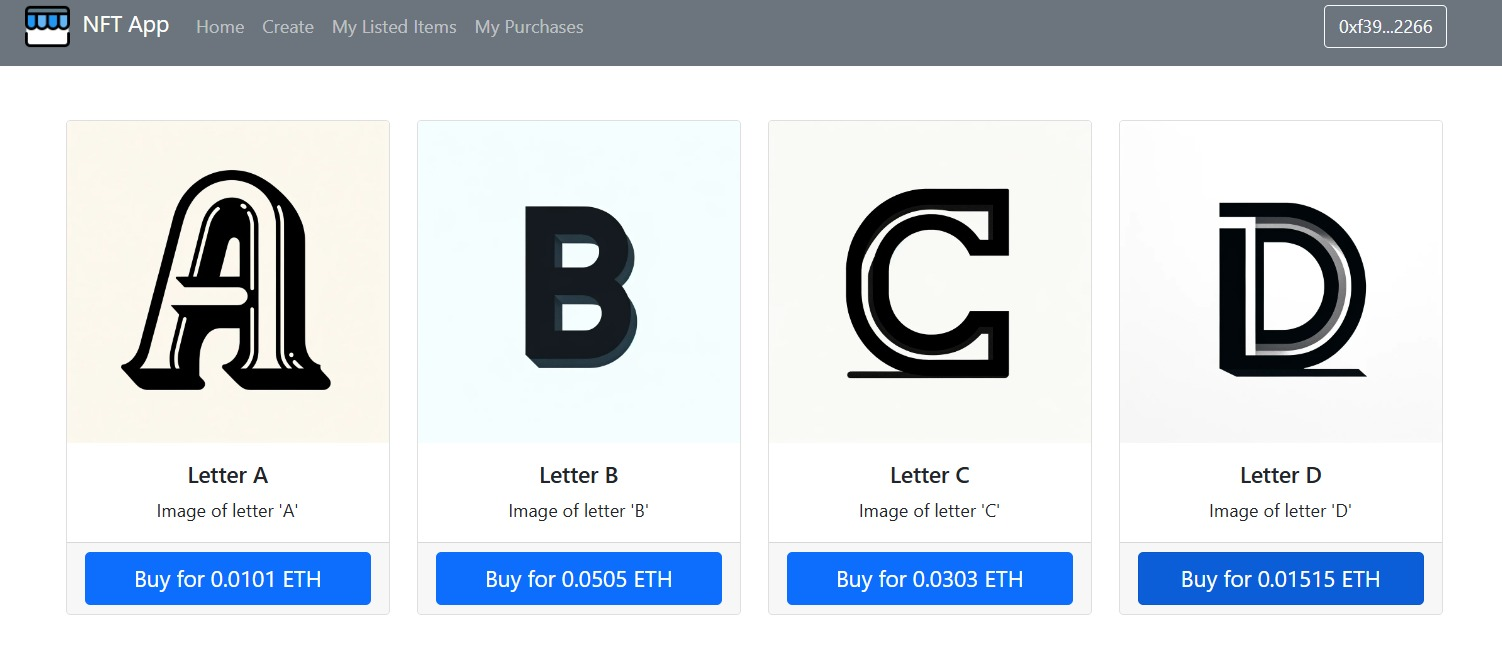
\includegraphics[scale=0.17]{gambar/tampilan_aplikasi.jpeg}
  % Caption for the image
  \caption{View of the web interface}
  % Reference label for the image
  \label{fig:web_view}
\end{figure}

\subsubsection{Smart Contract}
In the development of blockchain-based applications, integrating the smart contract with user interfaces such as React.js becomes crucial. The smart contract built using Solidity can be deployed on Ethereum testnets, such as the Sepolia Testnet, which provides an environment similar to the Ethereum mainnet but without requiring high transaction fees.

ABI, or Application Binary Interface, is a means that allows functions within an Ethereum smart contract to communicate with external applications, including user interfaces built with frameworks like React.js. ABI acts as a translation layer that outlines how to call functions in the smart contract, the types of parameters it accepts, the expected output types, and the state nature of those functions. ABI is typically generated automatically by the Solidity compiler as part of the smart contract compilation process and is stored in JSON format. Whenever the frontend application sends a transaction or query to the blockchain, it uses the ABI to encode the call data into a format that the Ethereum Virtual Machine (EVM) can understand. Then, when data is returned from the smart contract, ABI is used to decode the response so the React.js application can understand and process it.

The deployment process is carried out where the smart contract will be deployed to several blockchain networks, but for this testing, only the Sepolia testnet is used. During the deployment process, a gas or fee will be charged, which can be paid using Ethereum in the Metamask wallet. Details of this transaction can be seen on Etherscan.

\begin{figure} [H] \centering
  % Name of the image file
  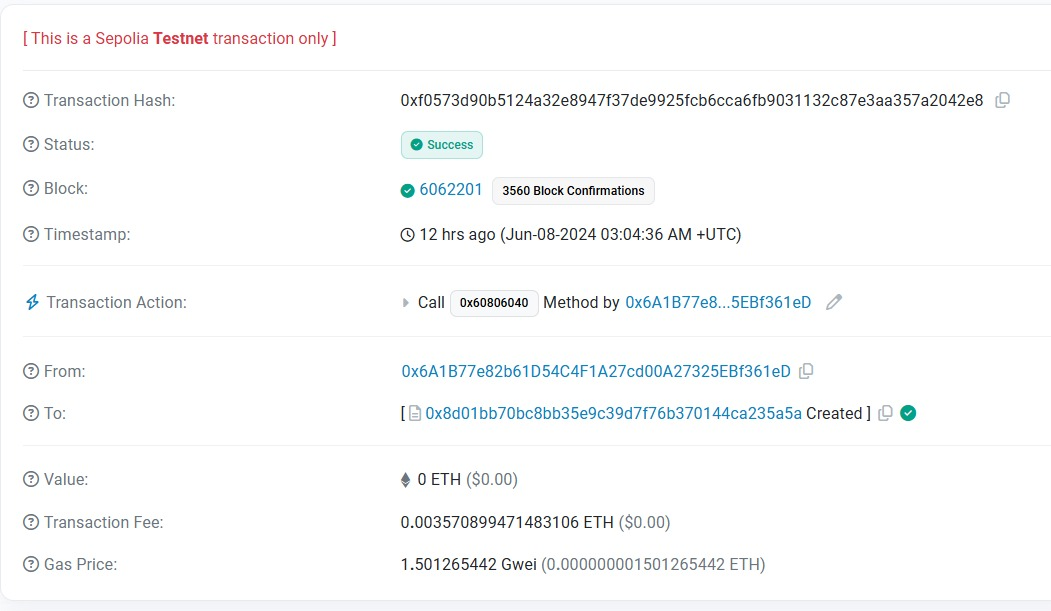
\includegraphics[scale=0.24]{gambar/etherscan.jpeg}
  % Caption for the image
  \caption{Transaction details on Etherscan}
  % Reference label for the image
  \label{fig:transaction}
\end{figure}

\subsubsection{Non-Fungible Token (NFT)}
Non-Fungible Tokens (NFT) also undergo several stages before they can be stored in The Interplanetary File System (IPFS) and then be published on OpenSea test net. In this thesis work, Pinata is used as a platform to upload NFT photos and JavaScript Object Notation (JSON) data so that it can be minted as a Uniform Resource Identifier (URI) on the smart contract. This is necessary so that the minted NFT has an image that can be viewed on OpenSea.

\begin{figure} [H] \centering
  % Name of the image file
  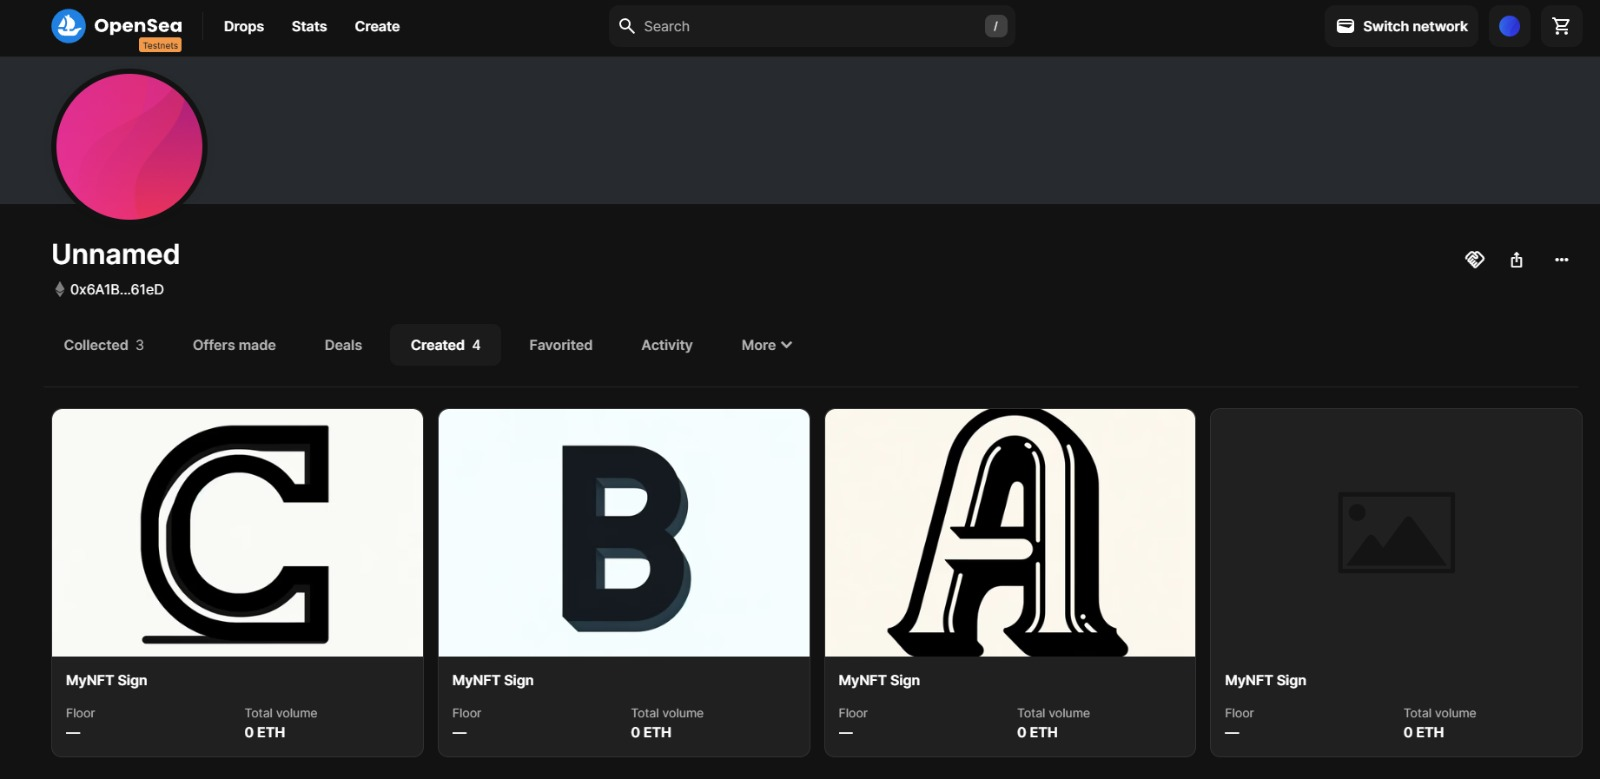
\includegraphics[scale=0.15]{gambar/opensea.jpeg}
  % Caption for the image
  \caption{NFT uploaded on Opensea}
  % Reference label for the image
  \label{fig:opensea}
\end{figure}

\subsection{Testing Features of Smart Contract Interoperability}
The testing expectations from the smart contract system include the following:
\begin{itemize}
    \item Users can mint NFT tokens, after which the ownership of these NFTs can be viewed on the test net platform OpenSea.

    \item Users from different Networks can communicate with each other, and the ownership of the NFT tokens can move from user A on network A' to user B on network B'.
\end{itemize}

Here is the data regarding the wallet used in testing:

\begin{table}[htbp]
  \centering
  \caption{Volume EDV dan ESV antara ground truth dan prediksi}
  \label{tab:volume}
  \scalebox{1.2}{
    \begin{tabular}{|c|p{2cm}|p{2cm}|}
      \hline
      \textbf{Account} & \textbf{Address} & \textbf{Network}
      \\
      \hline
      A & 0x6A1B77e \newline 82b61D54C4 \newline F1A27cd00A27 \newline 325EBf361eD & Sepolia \newline Ethereum \newline Testnet
      \\ 
      \hline
      B & 0xD066d6576 \newline D9485Eb2
      \newline c2a41BB8B52EcE \newline 17a0557d6 & BNB \newline Chain \newline Testnet \\
      \hline
      \end{tabular}    
  }
\end{table}

The following are the steps of testing the smart contract system that will be conducted:

\begin{itemize}
    \item User A will mint an NFT first

    \begin{figure} [H] \centering
    % Name of the image file
    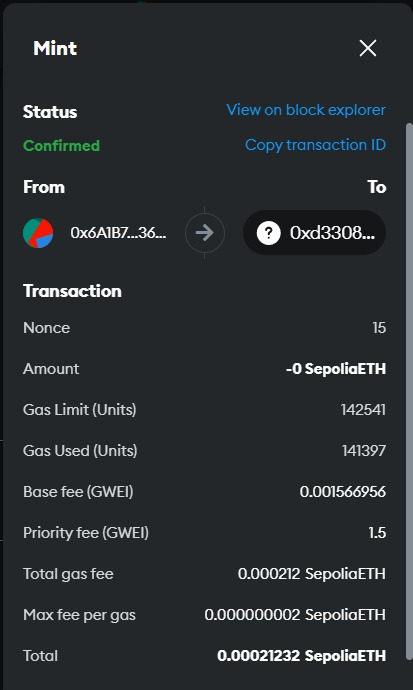
\includegraphics[scale=0.23]{gambar/riwayat_transaksi.jpeg}
    % Caption for the image
    \caption{Minting transaction history on Metamask Wallet}
    % Reference label for the image
    \label{fig:minting}
    \end{figure}

    \item The details on Etherscan can also be seen in the image below, showing details like the transaction hash, block, and the type of token, which is ERC-721.

    \begin{figure} [H] \centering
    % Name of the image file
    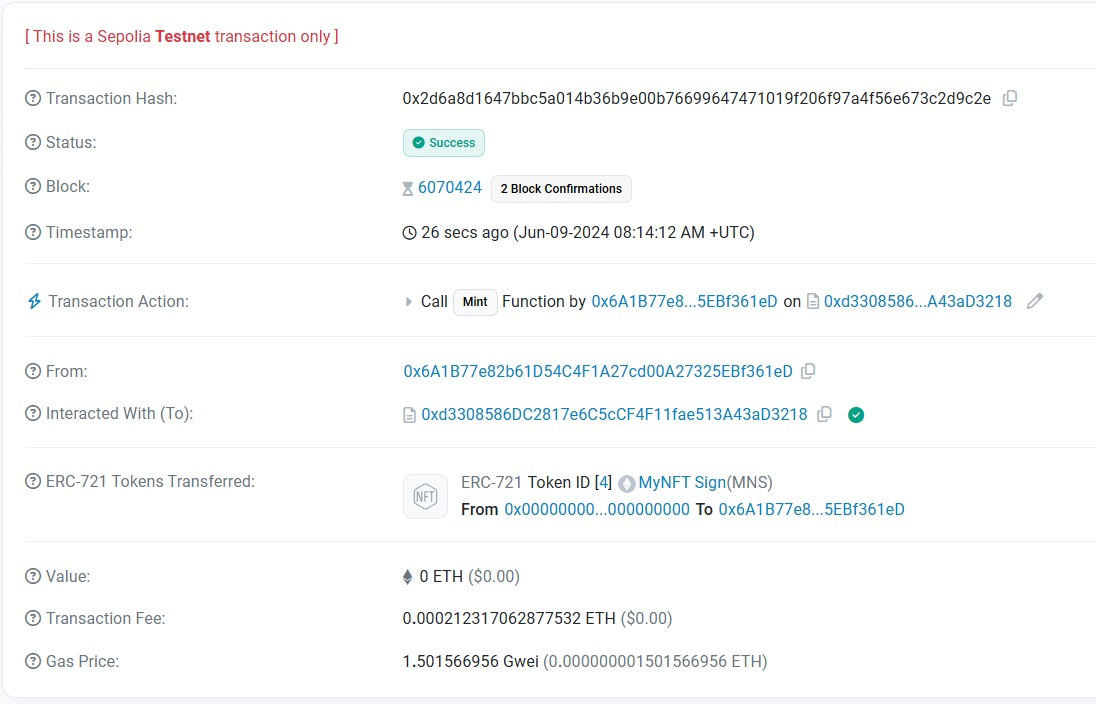
\includegraphics[scale=0.2]{gambar/detail_transaksi_etherscan.jpeg}
    % Caption for the image
    \caption{Transaction details on Etherscan}
    % Reference label for the image
    \label{fig:detail_transaction_etherscan}
    \end{figure}

    \item Then, on Etherscan, the details of the NFT that has been minted can be seen as in the following image

    \begin{figure} [H] \centering
    % Name of the image file
    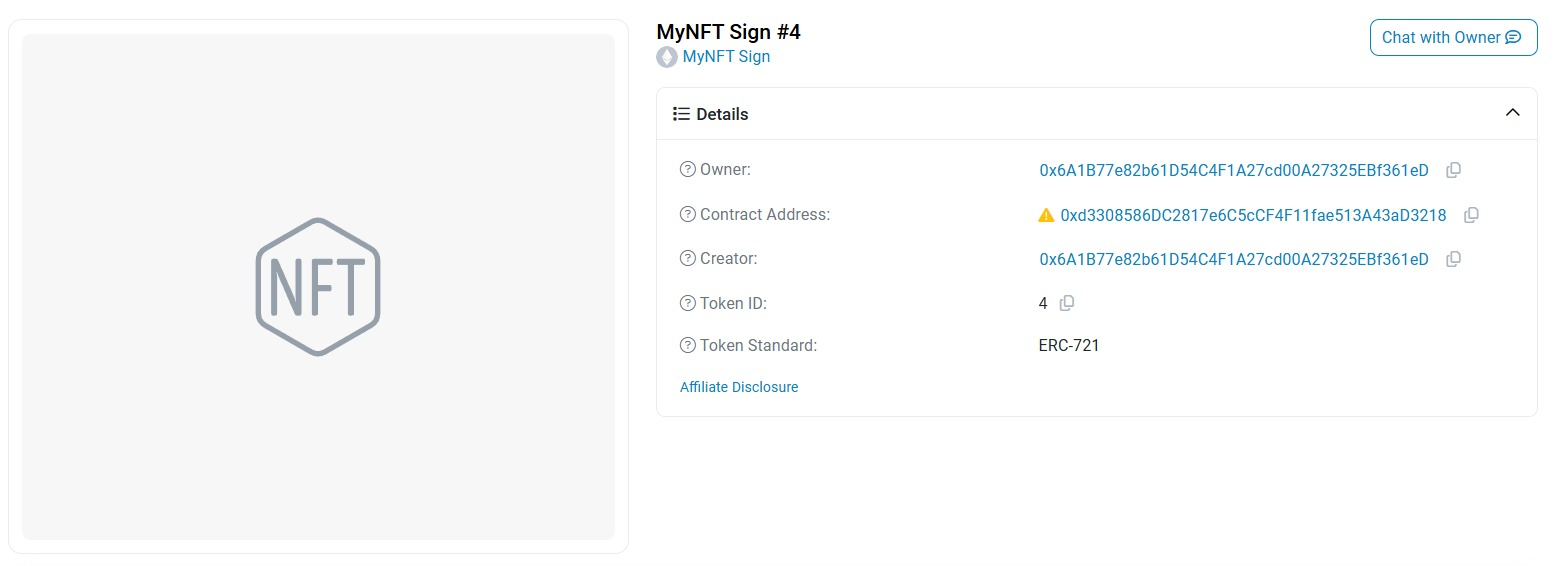
\includegraphics[scale=0.165]{gambar/detail_nft_etherscan.jpeg}
    % Caption for the image
    \caption{NFT Details on Etherscan}
    % Reference label for the image
    \label{fig:detail_nft_etherscan}
    \end{figure}

    \item After the process is successful, the NFT that has been minted can be seen on the platform OpenSea. In this test case, the minted NFT is "Letter D".

    \begin{figure} [H] \centering
    % Name of the image file
    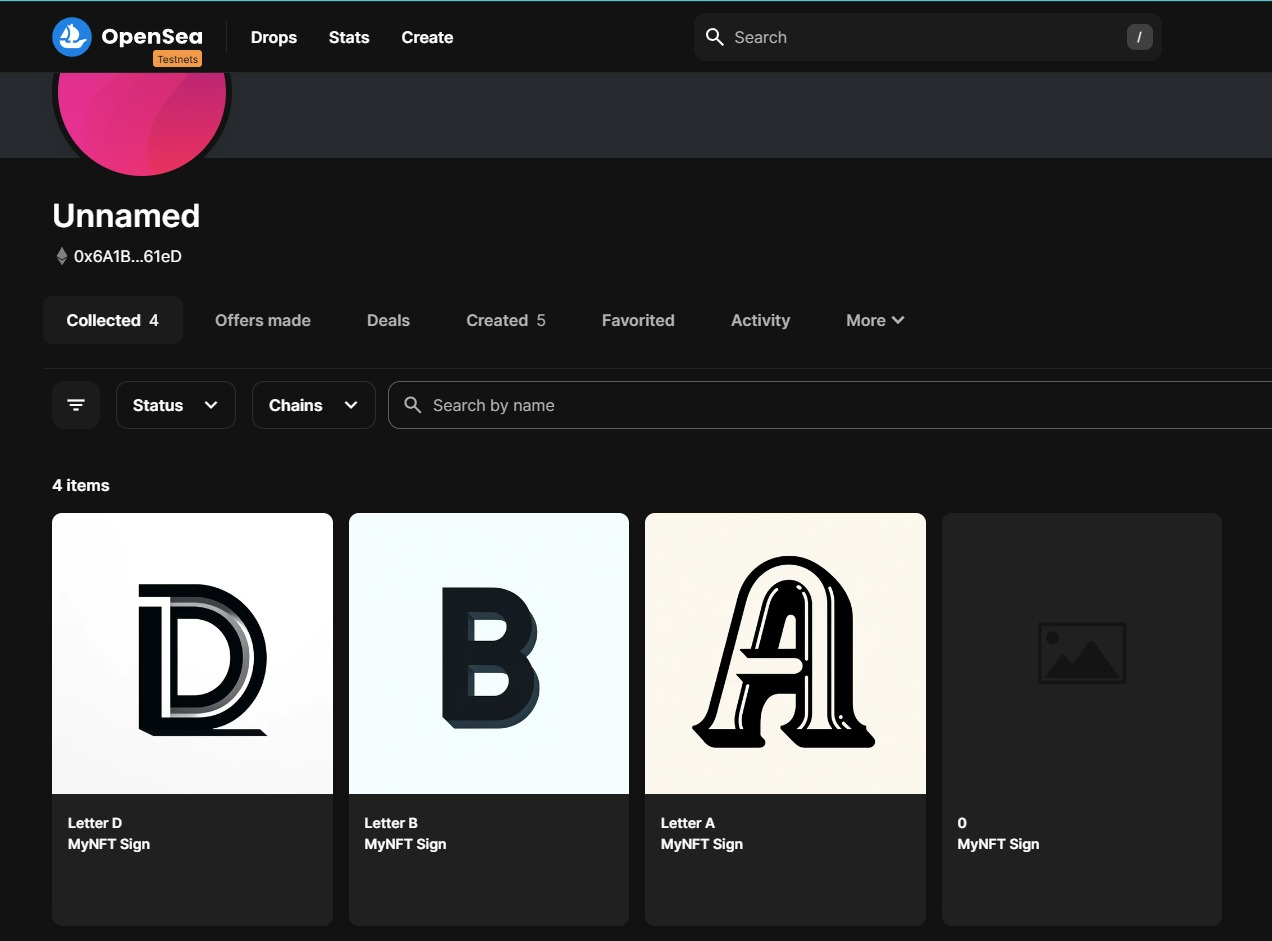
\includegraphics[scale=0.15]{gambar/nft_pada_opensea.jpeg}
    % Caption for the image
    \caption{NFT on OpenSea}
    % Reference label for the image
    \label{fig:nft_opensea}
    \end{figure}

    \item After the NFT is created, the next step is to lock the NFT to be sent to user B on network B'. The function of locking is to ensure that the token data is not changed during the transfer process, maintaining the trust and authenticity of the NFT data. It is also useful to signal to all related parties (users, smart contracts on other networks) that the token is undergoing a transfer process, and operations on the token should be suspended until the process is completed.

    \begin{figure} [H] \centering
    % Name of the image file
    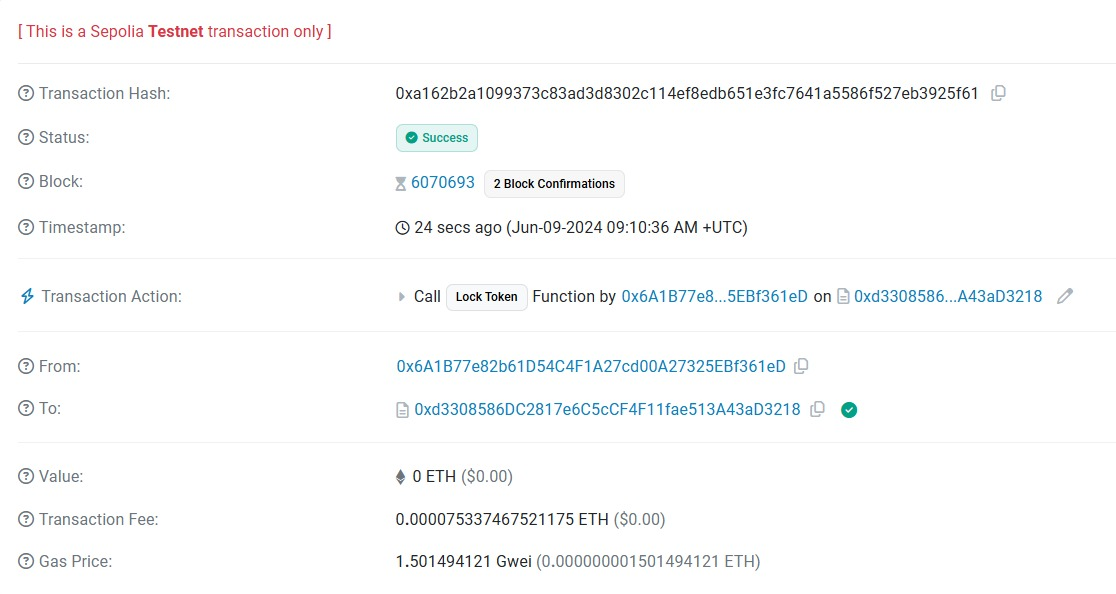
\includegraphics[scale=0.2]{gambar/lock_token.jpeg}
    % Caption for the image
    \caption{Lock Token function details on Etherscan}
    % Reference label for the image
    \label{fig:locktoken}
    \end{figure}

    \item After completing the lock token process, then the bridge transfer function can be executed. This function facilitates the secure transfer of NFTs between blockchains by ensuring that the NFT is locked during the transfer process and providing transparent visibility of the transfer event through recorded events. This is a key component in building interoperable applications that allow digital assets to move across blockchain ecosystems.

    \begin{figure} [H] \centering
    % Name of the image file
    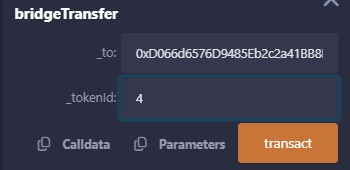
\includegraphics[scale=0.5  ]{gambar/bridge_transfer.jpeg}
    % Caption for the image
    \caption{Bridge transfer parameters}
    % Reference label for the image
    \label{fig:bridge_transfer}
    \end{figure}

    \item In the image \ref{fig:bridge_transfer}, there are two parameters: "\texttt{"\_to"}", used to receive the parameter address of user B, and "\texttt{"\_tokenId"}" to receive arguments from the NFT token. After the transaction is executed, it will be followed by payment on the Metamask Wallet.

    \begin{figure} [H] \centering
    % Name of the image file
    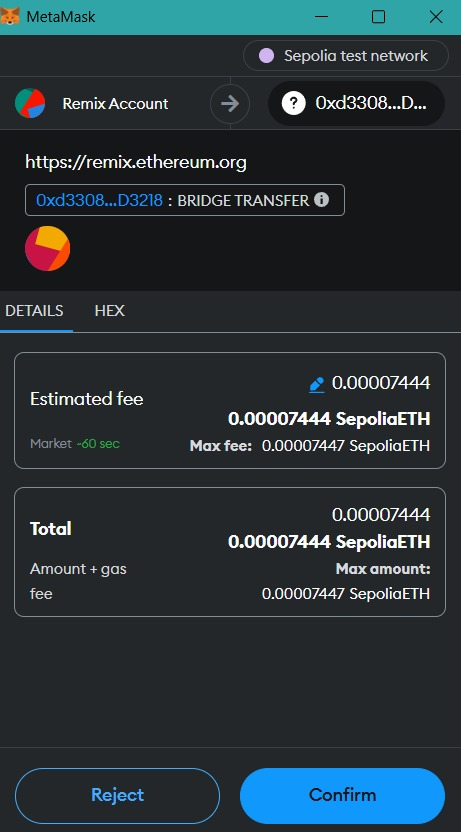
\includegraphics[scale=0.2]{gambar/verifikasi_metamask_wallet.jpeg}
    % Caption for the image
    \caption{Payment on Metamask Wallet}
    % Reference label for the image
    \label{fig:metamask_payment}
    \end{figure}

    \item After the transaction is successful, the record of the transaction is stored on the blockchain and can be viewed on Etherscan as shown in the image below.

    \begin{figure} [H] \centering
    % Name of the image file
    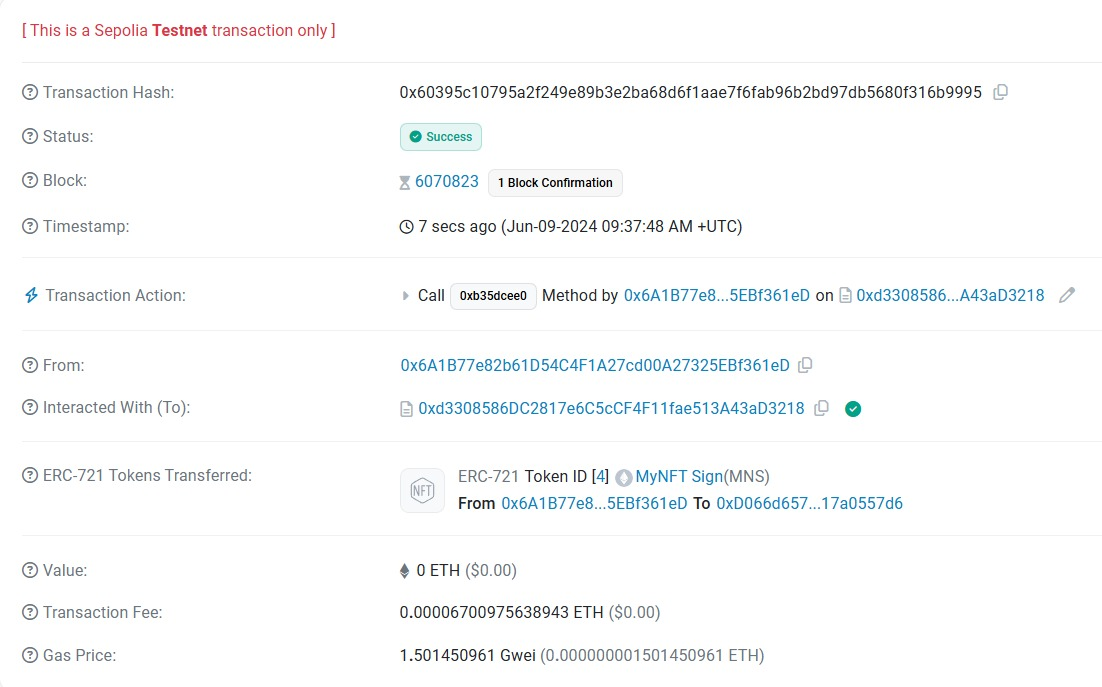
\includegraphics[scale=0.20]{gambar/detail_pada_etherscan.jpeg}
    % Caption for the image
    \caption{Details on Etherscan}
    % Reference label for the image
    \label{fig:details_etherscan}
    \end{figure}

    \item On Etherscan, details of the NFT can also be checked for ownership. As seen from the image \ref{fig:detail_nft_etherscan}, the owner of NFT \#4 is the address of user A on the Sepolia Ethereum Testnet, then in the image below, after successfully performing the bridge transfer, the ownership changes to user B on the BNB Chain Testnet.

    \begin{figure} [H] \centering
    % Name of the image file
    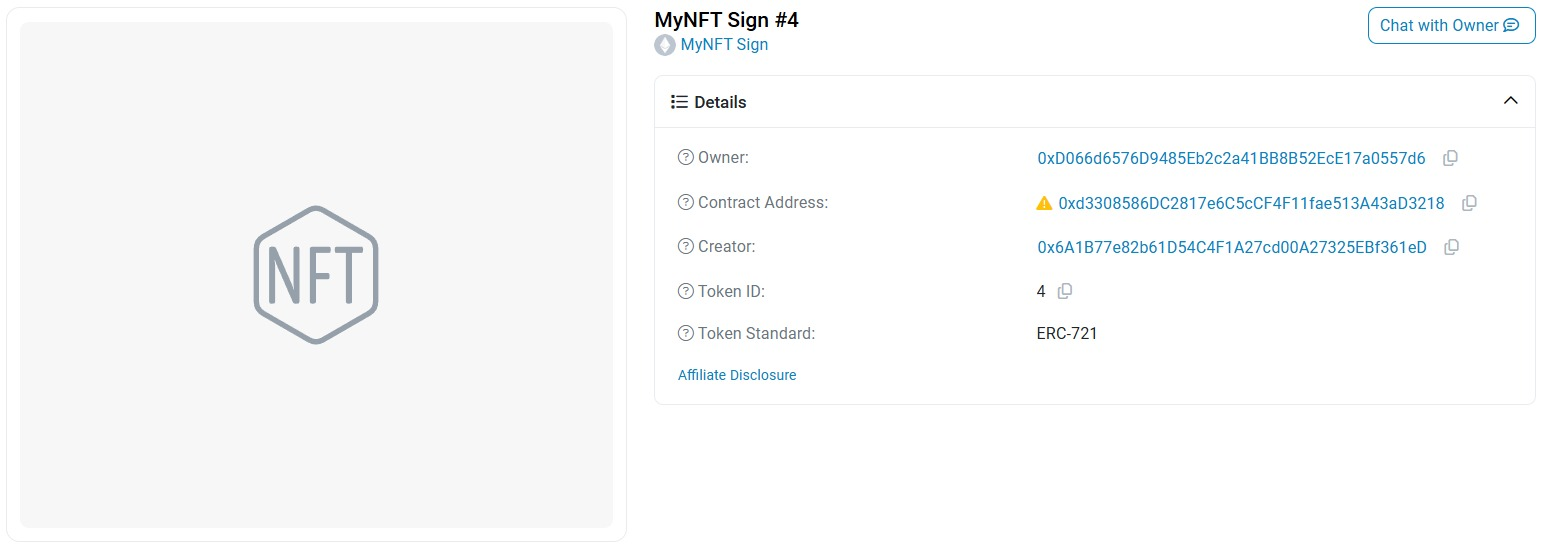
\includegraphics[scale=0.165]{gambar/nft_detail_etherscan2.jpeg}
    % Caption for the image
    \caption{NFT details on Etherscan after bridge transfer}
    % Reference label for the image
    \label{fig:nft_bridge_transfer}
    \end{figure}

    \item On the OpenSea platform, the NFT sent to the address of user B can also be seen.

    \begin{figure} [H] \centering
    % Name of the image file
    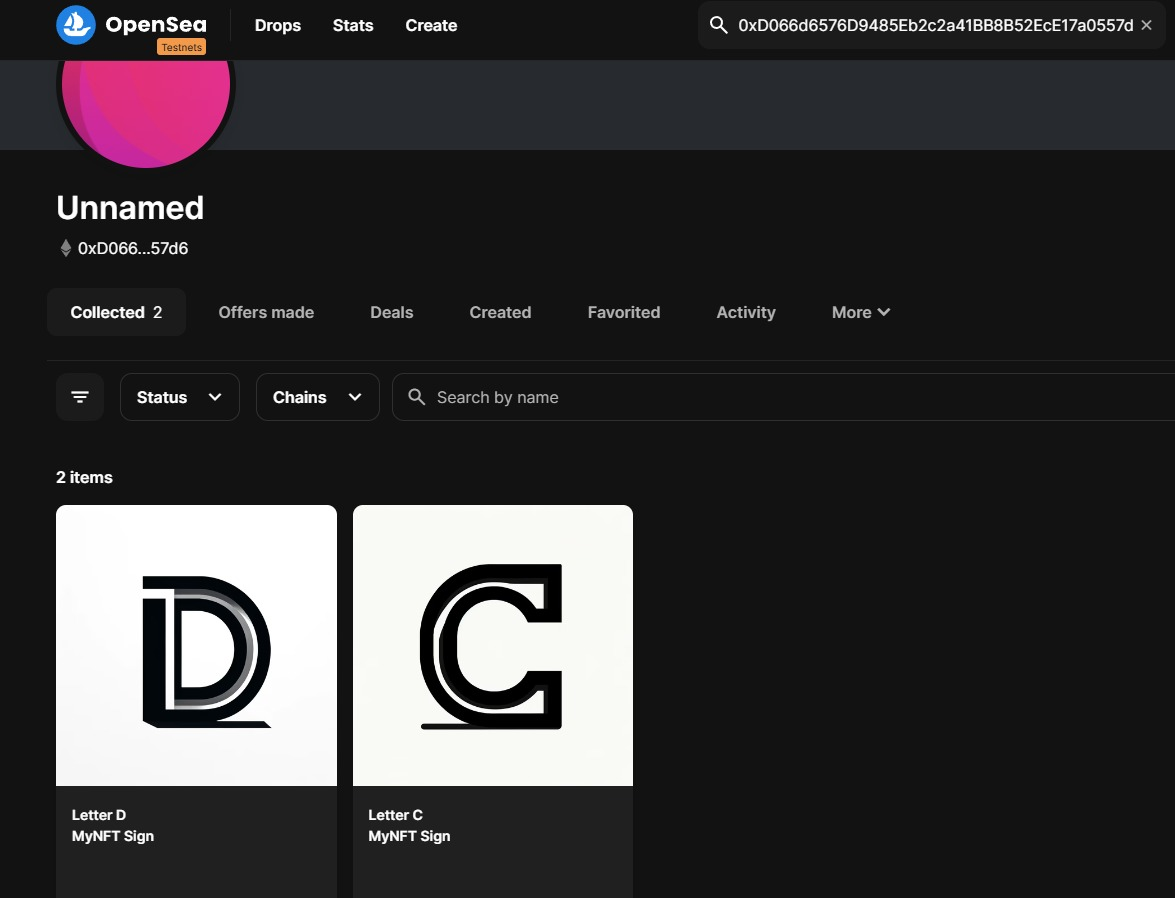
\includegraphics[scale=0.15]{gambar/nft_pada_opensea_2.jpeg}
    % Caption for the image
    \caption{NFT on OpenSea at the address of B}
    % Reference label for the image
    \label{fig:opensea2}
    \end{figure}
    
\end{itemize}
